\documentclass[11pt]{article}

\usepackage[utf8]{inputenc}
\usepackage[T1]{fontenc}

\usepackage{amssymb}
\usepackage{amsthm}
\usepackage{amsmath}
\usepackage{mathtools}
\usepackage{mathabx}
%\usepackage{framed}
\usepackage{booktabs}
\usepackage{hyperref}
\usepackage{txfonts}
\usepackage{siunitx}



\hypersetup
	{ 
		colorlinks=true,       % false: boxed links; true: colored links
%		hidelinks,
		linkcolor=blue,          % color of internal links (change box color with linkbordercolor)
		citecolor=green,        % color of links to bibliography
		filecolor=magenta,      % color of file links
		urlcolor=cyan,           % color of external links
		linkbordercolor	= {1 0 0},
		citebordercolor	= {0 1 0},	
		urlbordercolor	= {0 1 1}
	}


%\usepackage{fontspec}
%\setmainfont{Clear Sans}
%\newfontfamily{\clearsans}{Clear Sans}

\newcommand{\definition}{\\ \textbf{Definition:} \hspace{1cm} }

\newcommand*{\QEDA}{\hfill\ensuremath{\blacksquare}}%
\newcommand*{\QEDB}{\hfill\ensuremath{\square}}%


\begin{document}
	\title{Kapitel 14 - Statische elektrische Felder}
		\author
		{Johannes Bilk
			\\
			{\small 	\texttt{me@talachem.de}}
		}
		\date{\today}
	\maketitle
	\tableofcontents
	\setcounter{section}{13} %Hier f\"{a}ngt die Nummerierung an.
	
	\newpage
	
\section{Statische Elektrische Felder}	
	\subsection{ Elektrische Ladungen }	
	
	$\rightarrow$ Ab dem 17. Jahrhundert: Ursache für "elektrische Ph\"{a}nomene"; "neuartiger Stoff", elektrische Ladung
	
		\subsubsection{ Reibungselektriziz\"{a}t }
		
			\begin{itemize}
			\item Zwei Arten von "elektrischen Zust\"{a}nden" sind erzeugbar:
				\begin{itemize}
				\item Gleichartige Zust\"{a}nde $\implies$ Abstoßung
				\item Ungleichartige Zust\"{a}nde $\implies$ Anziehung
			\end{itemize}
			\item Carles Du Fay (1730): positiv/negativ elektrische Ladung
			\item Benjamin Franklin (1750): Über-/Unterschuss an "elektrischen Fluiden"
			\item Lichtenberg (1778): Zuordnung der Polari\"{a}t
			\end{itemize}
			
			\fbox{\begin{minipage}{19em}
			Hargummi stab: reiben mit Pelz, Wolle: -\\
			Glas, Plexiglas: reiben mit Seide: +
			\end{minipage}}
			\linebreak\\
			Reibezeug: entgegengesetzte Polarit\"{a}t
			$\implies$ Ladungstrennung, nicht etwa Ladungserzeugung.
			\linebreak\\
			Grunds\"{a}tzliches Messprinzip: Elektroskop: \hfill \\
			
			$\rightarrow$ Elektrometer $\rightarrow$ quantitative Messung
			\begin{itemize}
				\item "L\"{o}ffeln"; d.h. portionsweise Übertragung von Ladungen ist mglich
				\item Elektropendel: $\implies$ periodisches Umladen eines "Kugelpendel"
			\end{itemize}
			
			\subsubsection{Ladung ist eine skalare Gr\"{o}\ss{}e } Einheit 1C = 1 Coulomb, SI
				\begin{itemize}
					\item Zu jedem geladenen Elementarteilchen gibt es ein Elementarteilchen mit entgegengesetzter Ladung ($\rightarrow$ Ladungssymmetrie)
					\item Die Gesamtladung eines abgeschlossenen Systems bleibt erhalten ($\rightarrow$ Ladungserhaltung)
					\item Beispiel: Produktion eines $ e^+e^- $-Paares; $ E_\gamma \geq $ 1,02 MeV
				\end{itemize}
				
				\newpage
				
				\noindent Nachweis: Blasenkammer im Magnetfeld:  \hfill \\
				Umkehrung: "Zerstrahlung" von Positronen; $E=m\cdot c^2$
				\begin{itemize}
					\item Ladungtr\"{a}ger haben stets eine Masse
					\item Ladung kann nicht (im Gegensatz zur Masse) in Energie umgewandelt werden, bleibt auch bei Zerfallsprozessen erhalten.
					\item Quantisierung der Ladung: Alle in der Natur vorkommenden Ladungen sind ganzzahlige Vielfache der Elementarladung: $e_0:=1,602\cdot10^{-19}C; 1C=1AS$
				\end{itemize}
				\subparagraph{Beispiele von Ladungen}
				\begin{itemize}
					\item Neutral: $\gamma, \nu, n$
					\item einfach geladen: $e^-,e^+,p, \bar{p}$
					\item zweifach geladen:: $He_2(2^+,Z:2)$
				\end{itemize}	
				
\newpage

\subsubsection{ Quarks }	
\paragraph{Seit 60er Jahre}
Nukleonen bestehen aus Quarks, diese haben "drittelzahlige Ladungen"
\\
Up-Quarks:$u:+\frac{2}{3	}e_0$
\\
Down-Quarks:$d:-\frac{1}{3}e_0$
\\
Proton:$2u+d: 1\cdot e_0$
\\
Neutron:$u+2d: 0\cdot e_0$
\\

Quarks treten immer in 2er- oder 3er- Kombinationen auf.
\\

\subsubsection{Entdeckung und Bestimmung der Elementarladung}

Robert Andrews Millikan(1868-1953): Öltrpfchenversuch ($\rightarrow$ Anf\"{a}ngerpraktikum)


\subsection{Kr\"{a}fte zwischen Ladungen und das Coulomb-Gesetz} 

Charles-Augustin de Coulomb (1736-1806)

1785: Messung der Kraft zwischen zwei Ladungen als Funktion des Abstands mit Hilfe einer Torsionswaage \hfill \\

$$ \boxed{\vec{F_{12}} = f\cdot\frac{Q_1\cdot Q_2}{r^2_{12}}\cdot\frac{\vec{r_{12}}}{|\vec{r_{12}}|} = f\cdot\frac{Q_1\cdot Q_2}{r^2_{12}}\cdot \hat{r}_{12}} $$

\noindent F ist definiert durch die Definition der Ladungseinheit:
\\
Internationales Messsystem (SI): $f=\frac{1}{4\pi\epsilon_0}$
\\
$\epsilon_0=8,854\cdot10^{-12}\frac{(As)^2}{Nm^2}$
\\
ist Dielektrizit\"{a}tskonste des Vakuums oder elektrische Feldkonstante
\\
$Q_1\cdot Q_2 > 0:$ Abstoßung
\\
$Q_1\cdot Q_2 < 0:$ Anziehung

\subsection{Potenzielle Energie einer Ladungsverteilung}

...

\subsection{Erzeugung el. Felder durch Ladungen}

	\subsubsection{Feld einer Punktladung:}
	
	\begin{align*}
		\vec{F} &= \frac{1}{4\pi\epsilon_0} \cdot \frac{q_1 q_2}{ |\vec{r}_{12}|^2 } \cdot \hat{r_{12}} \\
					&=q_1 \underbrace{ \cdot \frac{1}{4\pi\epsilon_0} \cdot \frac{q_2}{ |\vec{r}_{12}|^2 } \cdot \hat{r_{12}}  }_{\text{Feld von }q_2} \\
					&=q_1 \vec{E}(\vec{r})
	\end{align*}
	\begin{itemize}
		\item Felder einer Punktladung sind Zentralfelder mit Kugelsymmetrie
		\item Konvention: Feldlinien führen von positiver zu negativer Ladung
	\end{itemize}
	\begin{center}
		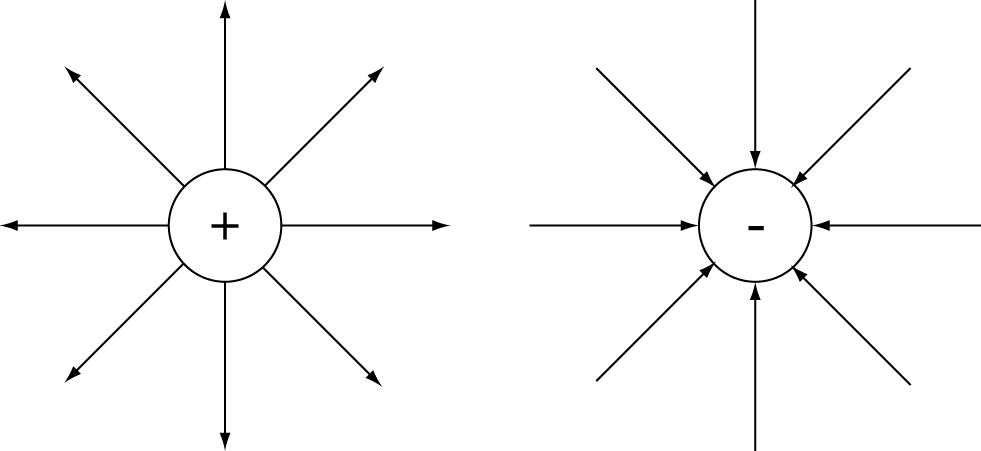
\includegraphics[width=0.7\linewidth]{skizzen/14/14_4B0}
	\end{center}

	$ \Rightarrow $ \underline{Punktladungsfelder sind inhomogen!}
	
	\subsubsection{Feld einer Verteilung von Punktladungen}
	N Ladungen bei $ \vec{r_i} $ 
	$$ \vec{E_i}(\vec{r}) = \frac{1}{4\pi\epsilon_0} \cdot \frac{q_i}{ | \vec{r} - \vec{r_i} |^2 } \cdot \frac{ \vec{r} - \vec{r_i}  }{ | \vec{r} - \vec{r_i}| }  $$
	Ungestörte Superposition:
	$$  \vec{E}(\vec{r}) = \frac{1}{4\pi\epsilon_0} \cdot {\displaystyle \sum_{i=1}^{N} \frac{q_i}{ | \vec{r} - \vec{r_i} |^2 } } \cdot \frac{ \vec{r} - \vec{r_i}  }{ | \vec{r} - \vec{r_i}| } $$
	\begin{minipage}{\textwidth}
		
		2 Ladungen, q ; -q : Feld eines Dipols 
		\begin{center}
			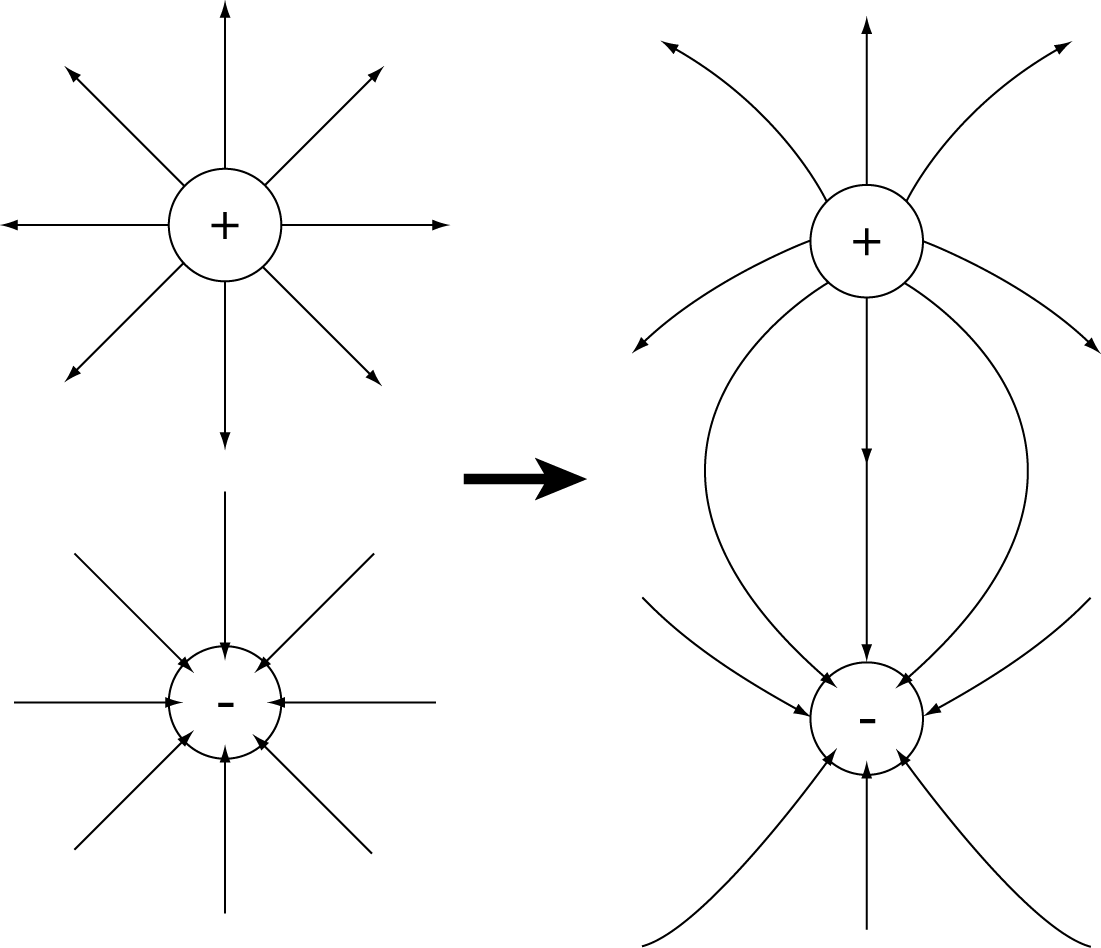
\includegraphics[width=0.4\linewidth]{skizzen/14/14_4B1}
		\end{center}
	
		2 Ladungen: q ; q 
		\begin{center}
			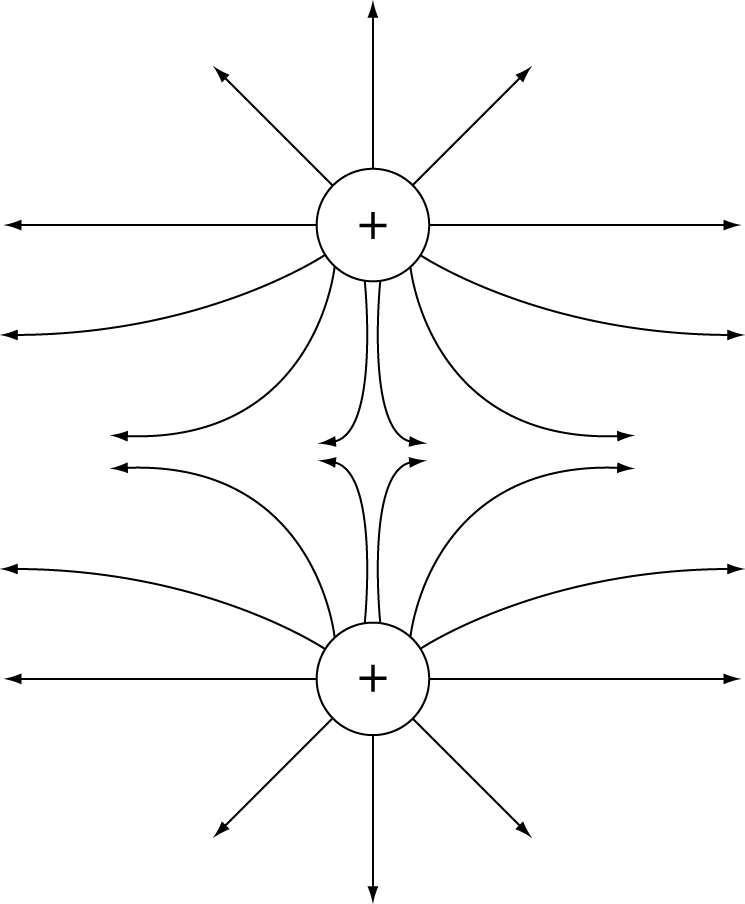
\includegraphics[width=0.4\linewidth]{skizzen/14/14_4B2}
		\end{center}
	
	\end{minipage}
	
	\begin{minipage}{\textwidth}
	
		Beispiele für "natürliche Dipole": \\
		\begin{enumerate}
			\item Neutrales Atom im homogenen $ \vec{E} $-Feld  
			\begin{center}
				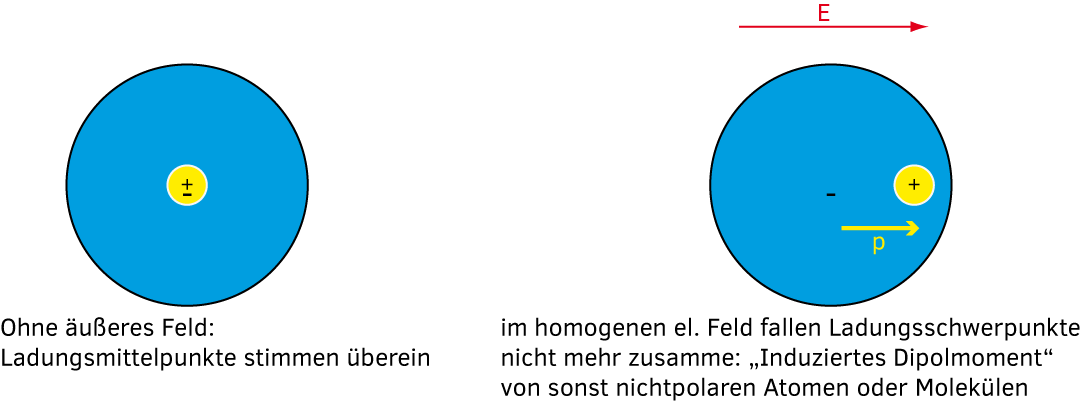
\includegraphics[width=0.9\linewidth]{skizzen/14/14_4B3}
			\end{center}
	
			\item Polare Molekühle mit permanentem Dipolmoment
			\begin{center}
				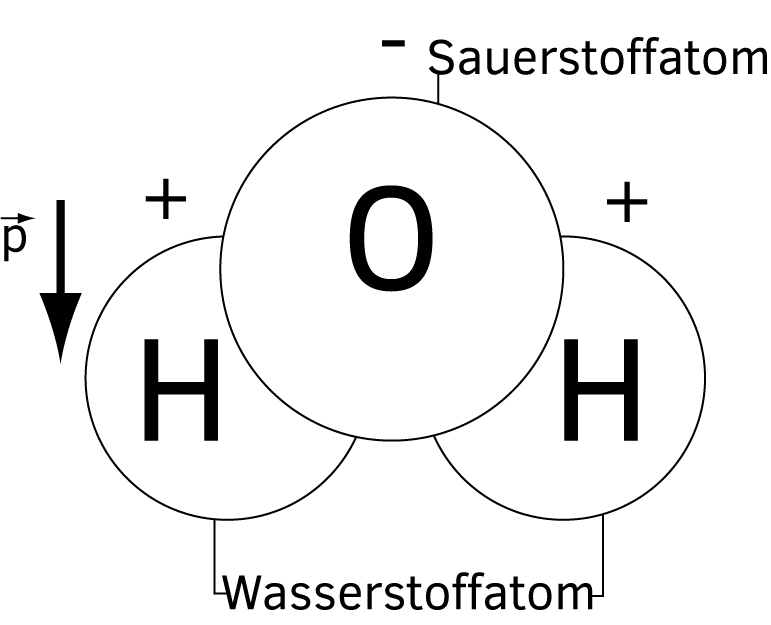
\includegraphics[width=0.4\linewidth]{skizzen/14/14_4B4}
			\end{center}
		
		\end{enumerate}
	
	\end{minipage}
	
	\subsubsection{Leiter im el. Feld und Influenz}
	Leiter: Ladungen sind \underline{frei} beweglich  \\
	Isolator: Ladungen sind ortsfest
	\begin{enumerate}
		\item $ \vec{E} = 0 $ im Inneren des Leiters 
		\begin{center}
			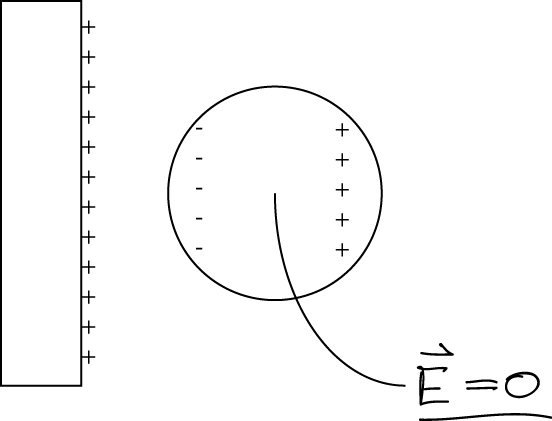
\includegraphics[width=0.4\linewidth]{skizzen/14/14_4B6}
		\end{center} 
		falls $ \vec{E} \neq 0 $: $ \vec{F} = q\vec{E} $ verschiebt Ladung bis $ \vec{E} = 0 $ ! 
		\item Es folgt, sich bei einem Leiter die (Netto-)Ladungen \underline{immer} an der Oberfläche befinden $ \Rightarrow $ Flächenladungsdichte $ \boxed{\sigma = \frac{dQ}{dA}} $
		\item $ \vec{E} $ immer $ \perp $ auf Leiteroberfläche
		\begin{center}
			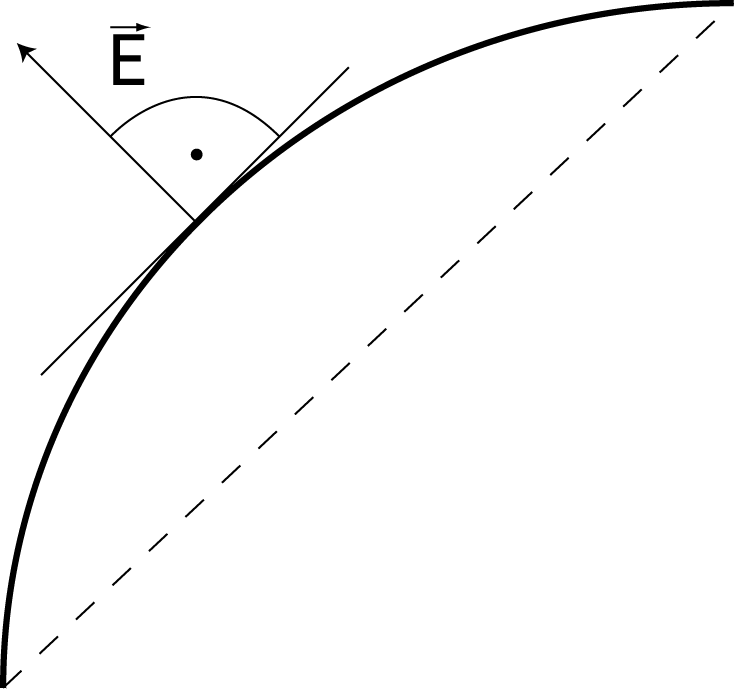
\includegraphics[width=0.4\linewidth]{skizzen/14/14_4B7}
		\end{center}
		(falls $ \vec{E}_{\shortparallel} \neq 0 $: Verschiebung der Ladung bis $ \vec{E}_{\shortparallel} = 0 $ !)

	\end{enumerate}
	\paragraph{\underline{Influenz}:} Räumliche Ladungstrennung in el. Leitern durch äu\ss{}eres $ \vec{E} $-Feld (Kontaktlos!), so dass das Innere des Leiters Feldfrei ist! 
	
	\subsection{Kontinuierliche Ladungsverteilung}
\end{document}
